\documentclass[11pt]{scrartcl}

\usepackage{graphicx}
\usepackage{amsmath}
\usepackage{wrapfig}
\usepackage{color}
\usepackage{sidecap}
\usepackage{listings}
\usepackage{syntax}
\usepackage{enumitem}
\usepackage[format=plain,indention=1em,margin=0.05\textwidth]{caption}

\newcommand{\unit}[1]{\ensuremath{\operatorname{#1}}}
\newcommand{\um}{\unit{\mu m}}
\newcommand{\declaration}[2]{\vspace*{2ex}#1\begin{addmargin}{1cm}{#2}\end{addmargin}}

\author{Peter Maunz}
\title{MQCO: Iontrapping experimental control software}

\begin{document}
\maketitle

\section{Overview}
The Trapped Ion Quantum Control System (IonControl) consists of FPGA controller hardware and a python computer frontend. On the FPGA (Opal Kelly XEM-6010) an enhanced van Neumann machine is executed which allows the user to control the experimental procedure in a powerful assembler like language.

\section{FPGA firmware}

%{\tiny
%\lstset{numbers=left, numberstyle=\tiny}
%\lstinputlisting{../prog/Ions-samples/ExternalScan.pp}
%}

The FPGA firmware executes a {\it Pulse Program}. The Pulse Program can be at most $4096$ words long where each command and variable take $1$ word of memory. The Pulse Program has access to the program memory in which variables are stored. Via simple commands there is also access to the on-board SDRAM (128 MByte). This memory can be written to and read from the host computer. In addition there are two pipes implemented between the host computer and the FPGA Pulse Program. Values can be read from and written to these pipes.

Counters to count incoming pulses are implemented in a gated setup. The Pulse Program sets the gates for the $24$ different counters, the counting is then done in parallel to the execution of the Pulse Program. When the gate is lowered, the accumulated counter value (24 bit) is transfered to the computer via the outgoing pipe without the intervention of the Pulse Program (only channels $0-15$). The counter value can also be read from the Pulse Program.

The are $8$ timestamping channels implemented. Currently, there are $8$ singal input routed to the counters. Counters $0-7$, $8-15$,$16-23$. 

The Pulse Program can be either written in an assembler like language or a higher level compiler level programming language.

\subsection{High-level program example}
The high-level language fromdefining a pulse program follows python syntax. Indentation defines blocks.

\definecolor{green}{rgb}{0,0.6,0}
\lstdefinelanguage{ppp}  
  { morekeywords={const,parameter,shutter,masked_shutter,counter,trigger,var,exitcode,def,while,if},
 morecomment=[l]{\#}
}
\newcommand*{\Comment}[1]{\hfill\makebox[0.5\textwidth][l]{\parbox{0.5\textwidth}{\color{green}#1}}}%
\lstset{language=ppp, columns=flexible, numbers=left, breaklines=true, commentstyle=\color{green}, breakindent=15em, escapechar=\&}
\begin{lstlisting}
#############################
# Gate Sequence Example

const DDSDetect = 1   &\Comment{\# constant definitions}&
const DDSMicrowave = 2
const PMTChannel = 9

# 397 beam frequencies and amplitudes
# parameter<encoding> name = value unit
parameter<AD9912_FRQ> DetectFreq = 100 MHz
parameter DetectAmp = 1023
parameter<AD9912_FRQ> MicrowaveFreq = 40 MHz
parameter<AD9912_PHASE> MicrowaveInitPhase = 0
parameter<AD9912_PHASE> MicrowaveAnalyzePhase = 0

# masks and shutters
shutter InitializationShutter   &\Comment{\# defines a shutter variable (digital outputs) with all bits masked on}&
masked_shutter CoolingOn   &\Comment{\# defines a shutter variable (digital outputs) and a mask variable}&
masked_shutter PumpingOn
masked_shutter MicrowaveOn
masked_shutter DetectOn

# times
parameter CoolingTime = 1 ms     &\Comment{\# parameters can be hcanged from the user interface}&
parameter PumpTime = 0 ms
parameter QubitInitTime = 0 us
parameter QubitAnalyzeTime = 0 us
parameter DetectTime = 1 ms
parameter AmplitudeSettlingTime = 100us
parameter gateTime = 100 us
parameter piTime = 90 us
parameter PostPulseWaitTime = 0us

# control parameters
parameter MaxInitRepeat = 10
parameter experiments = 100
counter CheckIonCounters   &\Comment{\# defines counter gates variable}&
counter DetectCounters
trigger ddsApplyTrigger     &\Comment{\# defines trigger output variable }&
trigger ddsMicrowaveApply
parameter PresenceThreshold 
parameter UseGateSequence

# internal variables
var currentExperiment &\Comment{\# defines a plain variable, which does not appear in the user interface}&
var initRemaining = 0
var trainPhase = 0
parameter trainTime = 0
var PulsesRemaining = 0
var RamStartAddress = 0

# exitcodes
exitcode IonLostExitcode = 0x1 &\Comment{\# exitcodes are only 16bit, the 16 MSB are 0xfffe  }&
exitcode endLabel = 0x0

# functions can be called for convenience, however, the language does not support function
# calls and all functions are inlined when called
def cool():          
    set_dds( channel=DDSMicrowave, freq=MicrowaveFreq )
    set_shutter( CoolingOn )
    set_counter( CheckIonCounters )
    update( CoolingTime )    &\Comment{\# update }&
    clear_counter()
    update( )
    set_inv_shutter( CoolingOn )
    W = load_count( PMTChannel )

def pump():
    set_shutter( PumpingOn )
    update( PumpTime )
    set_inv_shutter( PumpingOn )

def qubitInit():
    set_dds( channel=DDSMicrowave, phase=MicrowaveInitPhase )
    set_trigger( ddsMicrowaveApply )
    set_shutter( MicrowaveOn )
    update( QubitInitTime )
    set_inv_shutter( MicrowaveOn )

def qubitAnalyze():
    set_dds( channel=DDSMicrowave, phase=MicrowaveAnalyzePhase )
    set_trigger( ddsMicrowaveApply )
    set_shutter( MicrowaveOn )
    update( QubitAnalyzeTime )
    set_inv_shutter( MicrowaveOn )
    
def detect():
    set_dds( channel=DDSDetect, freq=DetectFreq )
    set_shutter( DetectOn )
    set_counter( DetectCounters )
    set_trigger( ddsApplyTrigger )
    update( DetectTime )
    set_inv_shutter( DetectOn )
    clear_counter()
    
# startup switching on cooling quickly
set_shutter( InitializationShutter )
set_dds( channel=DDSDetect, freq=DetectFreq, amp=DetectAmp )
set_trigger( ddsApplyTrigger )

while not pipe_empty():
    update()
    apply_next_scan_point()
    
    currentExperiment = 0
    while currentExperiment < experiments:
        set_ram_address( RamStartAddress )
        cool()
        if MaxInitRepeat>0: 
            initRemaining = MaxInitRepeat
            W = load_count( PMTChannel )
            while W<PresenceThreshold:
                if initRemaining==0:
                    exit( IonLostExitcode )
                cool()
        if PumpTime>0:
            pump()
        if QubitInitTime>0:
            qubitInit()         
        if UseGateSequence!=0:
            PulsesRemaining = read_ram()
            while PulsesRemaining!=0:
                PulsesRemaining -= 1
                trainPhase = read_ram()
                trainTime = read_ram()
                set_dds( channel=DDSMicrowave, phase=trainPhase )
                set_trigger( ddsMicrowaveApply )
                if trainTime!=0:
                    update(trainTime)
                trainTime = read_ram()
                if trainTime!=0:
                    set_shutter( MicrowaveOn )
                    update( trainTime )
                    set_inv_shutter( MicrowaveOn )
            update( PostPulseWaitTime )
        if QubitAnalyzeTime>0:
            qubitAnalyze()
        if DetectTime>0:
            detect()
        currentExperiment += 1  
        
exit( endLabel )
\end{lstlisting}

\subsection{Low-level program example}

\subsection{Pulse Program Basics}
The Pulse Program uses \lit{\#} as the rest of line comment character (python style comments). 

\declaration{\lit*{insert} \synt{filename}}{is used to insert the contents of one file at the position of the insert command.}

\declaration{\lit*{const} \synt{constant}}{is used to define constants. Constants have to be used for the \synt{channel} arguments of the DDS commands. In general if a command takes two arguments, the first argument has to be a constant.}

\declaration{\lit*{var} \synt{name}  \synt{value}, [\synt{type}], [\synt{unit}], [\synt{encoding}]}{ is used to declare variables.  For the Pulse Program only the \synt{name} and \synt{value} arguments are used. The additional arguments are interpreted by the graphical front-end to enable the control of the variable values. The \synt{type} defines what the intended use of the variable. The \synt{unit} describes it default dimension and unit. The \synt{encoding} determines how a variable value which on the front-end side can be a floating point value with physical quantity is converted into the 32 bit binary value used on the FPGA.

The possible types are 
\begin{description}
\item[\lit*{parameter}] The variable will be used as a parameter variable.
\item[\lit*{exitcode}] The variable will be used as an exitcode transmitted to the computer at the end of program execution.
\item[\lit*{trigger}] The variable will be used for trigger values.
\item[\lit*{mask}] The variable will be used as a bitmask to mark significant bits for a shutter value.
\item[\lit*{shutter} \synt{mask variable name}] The variable will be used as a shutter variable together with the bitmask \synt{mask variable name}.
\end{description}
Possible encodings are
\begin{description}
\item[\lit*{AD9912_FRQ}] The frequency value will be converted into the coarse frequency word for the AD9912 (32 most significant bits)
\item[\lit*{AD9912_FRQFINE}] The frequency value will be converted into the fine frequency word for the AD9912 (16 least significant bits)
\item[\lit*{AD9912_PHASE}] The value in degree will be converted  to the AD9912 phase word
\item[\lit*{CURRENT}]
\item[\lit*{VOLTAGE}]
\item[\lit*{TIME}] The time duration value will be converted into clock cycles.
\end{description}
Independent of the definition, variables with dimension time will always be converted to clock cycles.}

\declaration{\synt{label}\lit*{:}}{Is the declaration of a label. Jump command can set the next command to a label.}

\subsection{Basic commands}
The van Neumann machine uses two main internal registers. The W register is used to hold values while the INDF register holds the address of a variable. Basic command are available to load and store values from the memory into these registers. There are also commands to manipulate the W register.

\begin{addmargin}{1cm}
\begin{description}
\item[\lit*{NOP}] \hfill\\ 
  No operation

\item[\lit*{END}]  \hfill\\  
End execution.

\item[\lit*{LDWR} \synt{variable}] \hfill\\ 
 load value from variable into W register.

\item[\lit*{LDWI}]\hfill\\ 
load value from the address pointed to by INDF register into W register.

\item[\lit*{STWR} \synt{variable}] \hfill\\  
store value in W register into variable.

\item[\lit*{STWI}] \hfill\\  
store value from W register into address pointed to by INDF register.

\item[\lit*{LDINDF} \synt{variable}] \hfill\\  
load the contents of {\it variable} into the INDF register.

\item[\lit*{ANDW} \synt{variable}]  \hfill\\ 
 $W = W \& \text{{\it variable}}$.

\item[\lit*{ADDW} \synt{variable}]  \hfill\\  
$W = W +  \text{{\it variable}}$.

\item[\lit*{INC} \synt{variable}]  \hfill\\
$  W = \text{{\it variable}} + 1$.

\item[\lit*{DEC} \synt{variable}]  \hfill\\  
$W = \text{{\it variable}} - 1 $.

\item[\lit*{CLRW}]  \hfill\\  
$W = 0$.

\item[\lit*{ORW} \synt{variable}]\hfill\\  
Bitwise or. $ W = W | \text{\it variable}$.
\end{description}
\end{addmargin}

\subsection{Comparison and jumps}
Jumps can redirect the program flow to a \synt{label}. Depending on the jump command, a jump is conditioned either on the value of the W register or on the value of an internal compare bit. The internal compare bit is set by a comparison command.

\begin{addmargin}{1cm}
\begin{description}
\item[\lit*{CMP} \synt{variable}]  \hfill\\  
Set W to 0 if $W \le \text{{\it variable}}$ .

\item[\lit*{CMPEQUAL} \synt{variable}]  \hfill\\  
compare W and \synt{variable} and set the internal compare bit to true if $W=\synt{variable}$.

\item[\lit*{CMPNOTEQUAL} \synt{variable}]  \hfill\\  
compare W and \synt{variable} and set the internal compare bit to true if $W\neq\synt{variable}$.

\item[\lit*{CMPGE} \synt{variable}]\hfill\\  
compare W and \synt{variable} and set the internal compare bit to true if $W \ge \text{\it variable}$.

\item[\lit*{CMPLE} \synt{variable}]\hfill\\  
compare W and \synt{variable} and set the internal compare bit to true if $W \le \text{\it variable}$.

\item[\lit*{CMPGREATER} \synt{variable}]\hfill\\  
compare W and \synt{variable} and set the internal compare bit to true if $W > \text{\it variable}$.

\item[\lit*{CMPLESS} \synt{variable}]\hfill\\  
compare W and \synt{variable} and set the internal compare bit to true if $W < \text{\it variable}$.

\item[\lit*{JMP} \synt{label}] \hfill\\   
Unconditional jump to {\it label}.

\item[\lit*{JMPZ} \synt{label}]  \hfill\\  
Jump to {\it label} if W = 0.

\item[\lit*{JMPNZ} \synt{label}] \hfill\\   
Jump to {\it label} if W != 0.

\item[\lit*{JMPCMP} {\it label}] \hfill\\   
Jump to label if the internal compare bit is set.

\item[\lit*{JMPNCMP} {\it label}] \hfill\\   
Jump to label if the internal compare bit is not set.
\end{description}
\end{addmargin}

\subsection{Shutter and counter-gate subsystem}
There are $32$ shutter channels (digital output bits) and $32$ trigger channels (trigger digital output bits). Both are digital output bits with the difference that the trigger bits will be reset by the firmware after one clock cycle, while the shutter bits have to be set by the Pulse Program. In addition there are $32$ bits of counter gates. These are used to gate the $24$ counter and $8$ timestamping channels.

Shutter, trigger and counter gates are buffered in the Pulse Program. The commands setting the values only set an internal buffer. One of the two \lit{UPDATE} commands is then used to apply all the values of shutters, triggers and counter gates simultaneously.

For setting the shutter bits an internal mask is used. In this way it is possible to define a mask of bits that will be changed.
\begin{addmargin}{1cm}
\begin{description}
\item[\lit*{SHUTTERMASK} \synt{variable}]  \hfill\\  
Set internal register shutter\_mask to {\it variable}.

\item[\lit*{ASYNCSHUTTER} \synt{ variable}]  \hfill\\  
Update internal shutter register, bits set in shutter\_mask are updated with the bits from {\it variable}.

\item[\lit*{ASYNCINVSHUTTER} \synt{ variable}]  \hfill\\  
Update internal shutter register, bits set in shutter\_mask are updated with the inverted bits from {\it variable}.

\item[\lit*{COUTERMASK} \synt{ variable}]  \hfill\\  
Set the internal register with gate signals for the 24 counters and 8 timestampers. Bits 23:0 gate counters 23:0, bits 31:24 gate  timestamping on channels 7:0. The $8$ external input channels are used repeatedly. External input channel $0$ is routed to counter channels $0$, $8$, and $15$. The counts from channels $0 - 15$ are transmitted to the computer after the counter is gated low. Channels $16-24$ are only accessible from the Pulse Program. The timestamping channels are also operated by a gate. On the enabling edge of the gate the current values of a global counter (running at $50\unit{MHz}$) is transfered to the computer. Each detection event will then trigger the transmission of the current counter value. On counter overrun a overrun marker is written to the host computer. In this way, the total time of the gate is not limited.

\item[\lit*{TRIGGER} \synt{variable}] \hfill\\   
Set internal trigger register.

\item[\lit*{UPDATE}  \synt{variable}]  \hfill\\  
Update shutters, counter gates, triggers and start the delay counter with the value in\synt{variable}. The delay counter runs in the background while the subsequent commands of the Pulse Program are executed. It is necessary to wait for the expiration of the counter with the \lit{WAIT} command before the next \lit{UPDATE}.

\item[\lit*{UPDATEINDF}]\hfill\\  
As update, use the value pointed to by th INDF register for the wait time.

\item[\lit*{WAIT}] \hfill\\   
wait until the delay counter expires. Waits until the counter is expired. If no counter is running it will not wait. If the counter expired before reaching this command, execution continues.

\item[\lit*{LDCOUNT} \synt{counterchannel}]  \hfill\\  
load the last counter value from \synt{counterchannel} (needs to be \lit{define}d) into W register.

\item[\lit*{LDTDCCOUNT}]  \hfill\\  
load the value from the global timestamping counter into W.

\end{description}
\end{addmargin}

\subsection{Pipe from and to host computer}
The pipe to and from the computer allow efficient control of the Pulse Program and efficient transmission of results to the host computer. The pipes use $32$ bit words. In the case of the pipe to the computer, the most significant $8$ bits of the value are a marker for the $24$ data bits.

The following marker values are used:
\begin{addmargin}{1cm}
\begin{description}
\item[\lit*{0xffffffff}] end of experiment marker
\item[\lit*{0xfffexxxx}] exitcode marker with 16 bit exitcode 
\item[\lit*{0xff000000}] timestamping overflow marker
\item[\lit*{0xffffxxxx}] scan parameter with 12 bit address, is followed by additional scanparameter word.
\item[\lit*{0x1nxxxxxx}] $24$ bit count result from channel n (4 bit)
\item[\lit*{0x2nxxxxxx}] $24$ bit timestamp result channel n (4 bit)
\item[\lit*{0x3nxxxxxx}] $24$ bit timestamp gate start channel n (4 bit)
\item[\lit*{0x4xxxxxxx}] other return
\end{description}
\end{addmargin}

The following commands are used to interact with these pipes. Two consecutive commands accessing pipes need to be separated by commands that do not access pipes (e.g. \lit{NOP}).

\begin{addmargin}{1cm}
\begin{description}
\item[\lit*{WRITEPIPE}]  \hfill\\  
write the value in W into the pipe to the host computer. 

\item[\lit*{READPIPE}]  \hfill\\  
read a value from the pipe from the host computer into the W register. If there is no new data in the pipe, the last value in the pipe is used.

\item[\lit*{READPIPEINDF}]  \hfill\\  
Read the value from the pipe from the host computer in the INDF register.

\item[\lit*{WRITEPIPEINDF}]  \hfill\\  
Write the value from the INDF register into the pipe to the host computer.

\item[\lit*{JMPPIPEAVAIL}  \synt{label}]  \hfill\\  
Jump to \synt{label} if the pipe from the host computer has data.

\item[\lit*{JMPPIPEEMPTY} \synt{label}]  \hfill\\  
Jump to \synt{label} if the pipe from the host computer is empty.
\end{description}
\end{addmargin}

\subsection{Memory access}
It is possible to use the $128 \unit{MByte}$ of on-board SDRAM of the Opal Kelly module. However, while the FPGA block ram allows for random access in one clock cycle, the SDRAM has longer read and write latencies. As variables can be used for fast random access values, the use of the external memory is motivated by the need for large amount of memory. Usually, this memory is accessed in large junks. 

The memory framework thus uses a FIFO between SDRAM and Pulse Program. Consecutive values can be read from the FIFO in one clock cycle. Repositioning the memory pointer to a new (non-consecutive) values will clear the FIFO and start reading at the new location. There is a delay before the new data is available.

\begin{addmargin}{1cm}
\begin{description}
\item[\lit*{SETRAMADDR} \synt{variable}] \hfill\\  
Set the memory pointer to the address in {\it variable}.

\item[\lit*{RAMREADINDF}] \hfill\\  
Read one value from the RAM to the INDF register.

\item[\lit*{RAMREAD}]\hfill\\  
Read one value from the RAM to the W register.

\item[\lit*{JMPRAMVALID} \synt{label}]\hfill\\  
Jump to {\it label} if the RAM FIFO is valid.

\item[\lit*{JMPRAMINVALID} \synt{label}]\hfill\\  
Jump to {\it label} if the RAM FIFO is invalid.
\end{description}
\end{addmargin}

\subsection{Direct digital synthesizers}
The subsystem for the direct digital synthesizer  also uses a FIFO to allow for parallel data transmission to all DDS chips. The commands in the Pulse Program execute in one clock cycle. However, after execution, the command is not yet written to the DDS. For the AD9912 it takes approximately $2\unit{\mu s}$ to transmit one value (Phase, Frequency or Amplitude).

\begin{addmargin}{1cm}
\begin{description}
\item[\lit*{DDSFRQ} \synt{channel}, \synt{variable}] \hfill\\ 
write frequency (32 most significant bits) from variable to DDS channel. \synt{channel} has to be a define. The value is sent to the DDS in the background. It is only updated after an io\_update. 

\item[\lit*{DDSFRQFINE} \synt{channel}, \synt{variable}] \hfill\\ 
 write frequency (16 least significant bits) from variable to DDS channel.  \synt{channel} has to be a define. The value is sent to the DDS in the background. It is only updated after an io\_update. 

\item[\lit*{DDSAMP} \synt{channel}, \synt{variable}] \hfill\\ 
 write amplitude from variable to DDS channel. The value is sent to the DDS in the background and takes effect without io\_update. 

\item[\lit*{DDSPHS} \synt{channel}, \synt{variable}] \hfill\\ 
write phase from variable to DDS channel.  \synt{channel} has to be a define. The value is sent to the DDS in the background. It is only updated after an io\_update. 

\item[\lit*{WAITDDSWRITEDONE}]\hfill\\
Wait for the DDS writes to complete.

\end{description}
\end{addmargin}

\subsection{Deprecated commands}
These commands are only present for backwards compatibility and are not recommended to be used.
\begin{addmargin}{1cm}
\lit*{DDSCHN}, \lit*{SHUTTER}, \lit*{COUNT}, \lit*{COUNT1}, \lit*{COUNTBOTH}, \lit*{DELAY}, \lit*{STWR1}, \lit*{LDWR1}, \lit*{JMPZ1 }, \lit*{JMPNZ1}, \lit*{CLRW1}, \lit*{CMP1}
\end{addmargin}

\subsection{Common idioms}
\lstdefinelanguage{pp}  
  { morekeywords={NOP,JMPPIPEEMPTY,READPIPEINDF,WRITEPIPEINDF,READPIPE,WRITEPIPE,STWI,LDWR,STWR,END,
    JMP,JMPNZ,JMPZ,DEC,TRIGGER,SHUTTERMASK,ASYNCSHUTTER,WAIT,UPDATE,COUNTERMASK},
 morecomment=[l]{\#}
}
\lstset{language=pp, columns=flexible, numbers=left, breaklines=true, commentstyle=\color{green}, breakindent=15em, escapechar=\&}
Here I will list and describe common idioms used in Pulse Programs.

The idiom for generating a digital pulse pattern is the following:
\begin{lstlisting}
TRIGGER triggervariable   &\Comment{\# write the inteernal trigger buffer}&
SHUTTERMASK  maskvariable &\Comment{\# write the shutter mask}&
ASYNCSHUTTER shuttervariable &\Comment{\# update the shutter bits enabled in mask}&
COUNTERMASK countergates &\Comment{\# set the value for counter gates}&
WAIT &\Comment{\# wait for the last counter to expire}&
UPDATE timevariable &\Comment{\# update trigger, shutter and countermask and start the counter}&

TRIGGER triggervariable2   &\Comment{\# write the inteernal trigger buffer}&
SHUTTERMASK  maskvariable2 &\Comment{\# write the shutter mask}&
ASYNCSHUTTER shuttervariable2 &\Comment{\# update the shutter bits enabled in mask}&
COUNTERMASK countergates2 &\Comment{\# set the value for counter gates}&
WAIT &\Comment{\# wait for the last counter to expire}&
UPDATE timevariable2 &\Comment{\# update trigger, shutter and countermask and start the counter}&
\end{lstlisting}

The execution continues from line 6 to line 7 without waiting. Lines 8 to 11 do not affect the output of the FPGA. In line 12 we wait for the last counter of duration \lit*{timevariable} to expire. Then we continue to line 13.

An idiom to skip timesteps is realized in the following example. The example is for a step of waiting without changing any external settings.
\begin{lstlisting}
QubitWait: NOP	
	LDWR QubitWaitTime  &\Comment{\# load QubitWaitTime}&
	JMPZ QubitAnalyze    &\Comment{\# if time is 0 jump to next step}&
	WAIT   &\Comment{\# otherwise wait for last timer to expire}&
	UPDATE QubitWaitTime &\Comment{\# and update and set the new timer duration}&

QubitAnalyze: NOP
\end{lstlisting}

The jump commands can be used to condition the program execution on the measured results. In the following example for a ion cooling step, we are checking for the ion fluorescence. If we see enough counts, we continue, otherwise we repeat the cooling step. If the ion is not detected after a maximal number of steps we stop program execution.

\begin{lstlisting}
	LDWR MaxInitRepeat
	STWR initRemaining
cool: NOP
	SHUTTERMASK  CoolingOnMask &\Comment{\# set the mask of shutter to be changed for cooling}&
	ASYNCSHUTTER CoolingOn  &\Comment{\# set the shutter values}&
	COUNTERMASK CheckIonCounters &\Comment{\# set the counter gates}&
	WAIT &\Comment{\# wait for the last counter to expire}&
	UPDATE      CoolingTime &\Comment{\# update all values and start the cooling counter}&
	COUNTERMASK Null &\Comment{\# close all counter gates, leave cooling on}&
	WAIT  &\Comment{\# wait for end of cooling interval}&
	LDCOUNT	PMTChannel &\Comment{\# load the counter values (PMTChannel was defined as the number of the counter)}&
	CMP      	PresenceThreshold 	&\Comment{\# if counts greater than threshold W=W else W=0}&
	JMPNZ     	pump  		&\Comment{\# if ion detected go on in the sequence}&
	LDWR MaxInitRepeat &\Comment{\# Load the maximum number of repetitions}&
	JMPZ pump                       &\Comment{\#if MaxInitRepeat=0 disable the checking for an ion }&
	DEC initRemaining &\Comment{\# Decrease the number of cooling loops left}&
	STWR initRemaining &\Comment{\#Store the result}&
	JMPNZ cool  &\Comment{\# Retry if initRemaining is > 0}&
	LDWR IonLeftExitCode     &\Comment{\# Ion left, load the exitcode}&
	WRITEPIPE &\Comment{\# write the exitcode to the computer}&
	END &\Comment{\# End program execution}&
pump: NOP &\Comment{\# Here comes the next step}&
\end{lstlisting}


\section{Interfacing the Pulse Program with the frontend}
Currently the front-end uses two ways for scanning values between different experimental points. In the first case the FPGA is able to control all values that have to be changed during a scan. I will call this an {\em internal scan}, in the other case some external equipment controlled by the host computer has to be changed between between experimental points ({\em external scan}).

\subsection{Internal scan}
Because no host intervention is necessary for the internal scan, the whole scan can be executed with under Pulse Program control while the communication of results and scan values is done using the pipes. A typical Pulse Program would use the following idiom:

\begin{lstlisting}
scanloop: NOP
	JMPPIPEEMPTY endlabel   &\Comment{\# if no additional data is available in the pipe we are done with the scan}&
	READPIPEINDF  &\Comment{\# read the address of the variable to be changed from the pipe}&
	NOP
	WRITEPIPEINDF  &\Comment{\# write the address back to the computer as marker between different points}&
	NOP
	READPIPE   &\Comment{\# read the new variable value from the pipe}&
	NOP
	WRITEPIPE    &\Comment{\# write it back to the computer}&
	NOP
	STWI      &\Comment{\# store the new value in the variable}&
	LDWR experiments    &\Comment{\# load he number of experiments to do for this value}&
	STWR experimentsleft   &\Comment{\# store it in the loop parameter}&
experimentloop: NOP
\end{lstlisting}
 here goes everything that makes a single experiment. Please make sure to close counter gates and wait for the completion of the counter gate to ensure the results are assigned to the correct experimental point.

\begin{lstlisting}[numbers=left, firstnumber=last]
	DEC experimentsleft    &\Comment{\# decrease the number of experiments left to do, result is in W}&
	STWR experimentsleft &\Comment{\# store the result}&
	JMPNZ experimentloop        &\Comment{\# if experimentsleft>0 jump to experimentloop}&
	JMP scanloop     &\Comment{\# jump to scanloop}&
endlabel:
	LDWR myexitcode &\Comment{\# load exitcode into W register}&
	WRITEPIPE  &\Comment{\# write exitcode to pipe}&
	END &\Comment{\# end execution}&
\end{lstlisting}

\subsection{External scan}
For an external scan the FPGA only has to execute the experiments to be averaged into one result point. The Pulse Program is restarted for every point, however the Pulse Program is not overwritten for each point. Thus one needs to take care to not overwrite variables that will be needed in the next program run.

A minimal program could look like this:
\begin{lstlisting}
const COOLDDS 0
var startupMask       1, mask
var startup           1, shutter startupMask
var startupTime       1, parameter, ms
var coolingOnMask     1, mask
var coolingOn         1, shutter coolingOnMask
var coolingCounter    1, counter
var coolingOffMask    1, mask
var coolingOff        0, shutter coolingOffMask
var coolingOffCounter 0, counter
var coolingTime       10, parameter, ms
var experiments     350, parameter
var experimentsleft 350
var epsilon        500, parameter, ns
var endLabel 0xffffffff

	SHUTTERMASK startupMask
	ASYNCSHUTTER startup
	UPDATE startupTime
	LDWR experiments
	STWR experimentsleft
cooling: NOP
	SHUTTERMASK coolingOnMask
	ASYNCSHUTTER coolingOn
	COUNTERMASK coolingCounter
	WAIT                             # for end of startup or last
	UPDATE coolingTime

	SHUTTERMASK coolingOffMask
	ASYNCSHUTTER coolingOff
	COUNTERMASK coolingOffCounter
	WAIT
	UPDATE epsilon

	DEC experimentsleft
	STWR experimentsleft
	JMPNZ cooling	

	# write the end indicator
	LDWR endLabel
	WRITEPIPE	
	END

\end{lstlisting}


\section{Front-end}
The front-end is used to interact with the Pulse Program. It prepares the data to be written and analyzes the results from the Pulse Program. The main window (figure~\ref{MainWindow}) has controls for instruments while the Pulse Program is {\em not} running. The windows for the DDS, Shutters, Triggers and external instruments are all in separate dockwidgets. These dockwidgets can be re-arranged, torn out into an independent window or closed. Once closed they can be re-opend via the View menu or the contect menu of any dockwidget.

In addition to the Main window the program has non-modal windows for the Pulse Program configuration (pulse icon), the voltage control (Voltage icon), FPGA settings (gear icon), Logic analyzer (chip lupe icon). Furthermore, there is a "dedicated counters" window available from the graph icon. The separate windows are described in detail below.

\begin{figure}[htbp]
\begin{center}
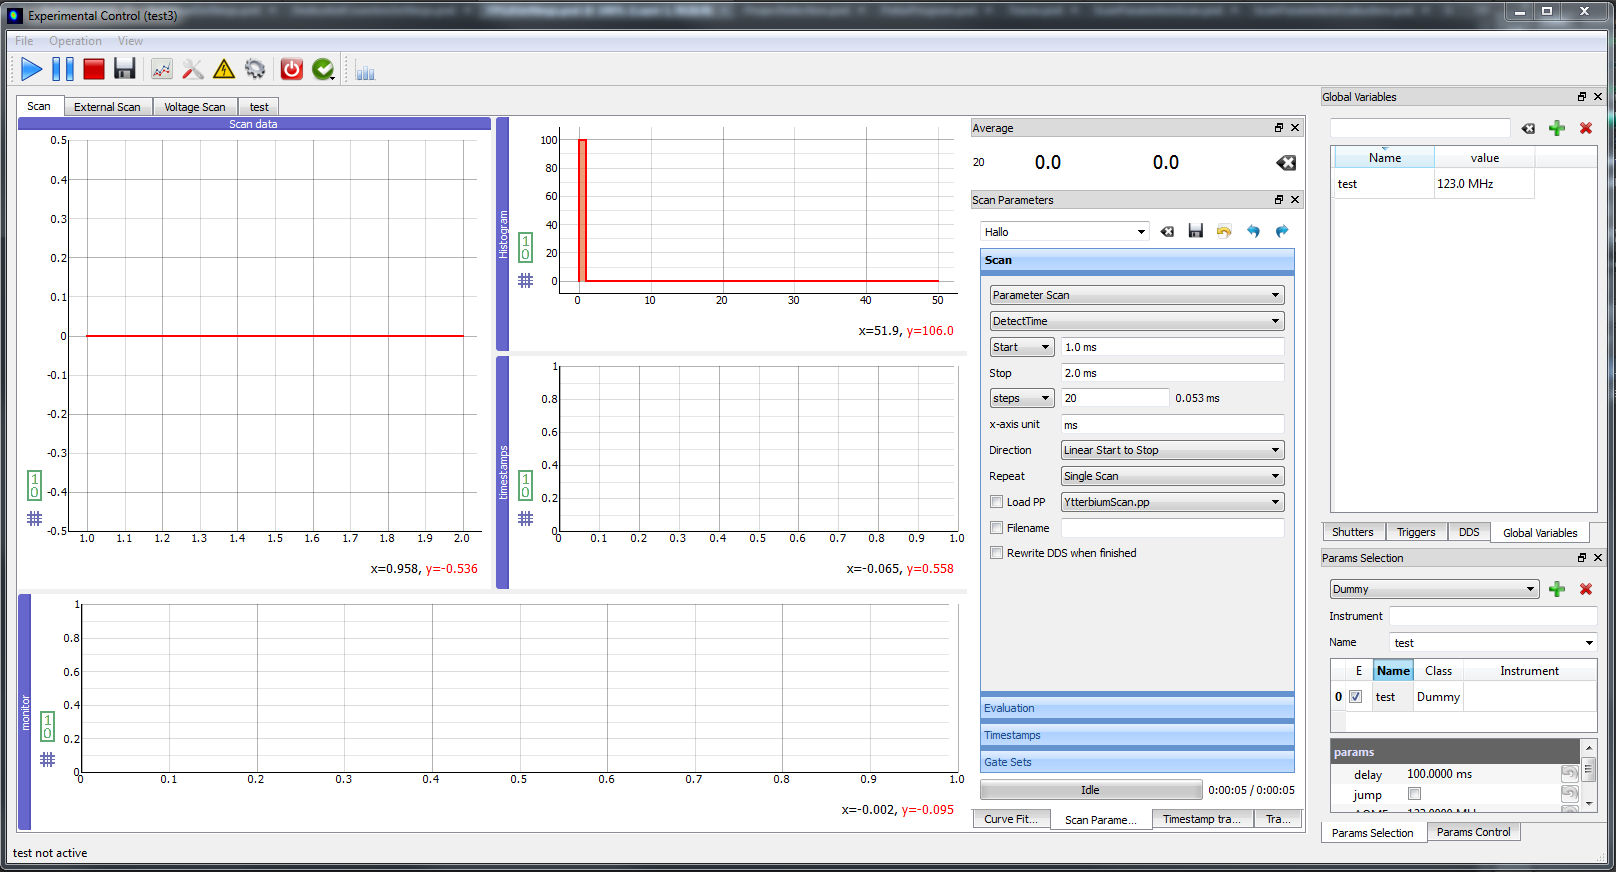
\includegraphics[width=\textwidth]{MainWindow}
\end{center}
\caption{\label{MainWindow} Main window. There two categories of dock widgets. Global variables, Triggers, Shutters, DDS, Params Selection, Pamams Control, Trace, Timestamp Tracee and Fit belong to the Main Window. The other visible dock widgets belong to active measurement.}
\end{figure}

\subsection{Project Selection}

\begin{SCfigure}
\centering
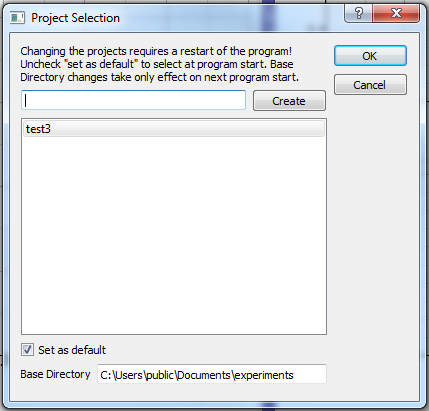
\includegraphics[width=0.48\textwidth]{ProjectSelection}
\caption{\label{ProjectSelection} Project Selection. Folders in the base directory are considered projects. All configuration data and result data is saved in the project folder.}
\end{SCfigure}

The control program defines a "Base directory". The folders in the Base directory are considered Projects. Each Project has dedicated gui settings and data directories. The configuration data of the control program is saved in the folder .gui-config in the Project directory. It is recommended to create a folder "config" for the pulse program files and other configuration files. Example files can be found in the {\em config} folder within the python source tree. Data is saved by default in a directory structure consiting of year, month and day directories. This window is shown on first startup of the control program.

If "Set as default" is checked the control program will start with the default project. In this case the project can be changed by selecting File $\rightarrow$ Project. Changing the Project requires an immediate restart of the program.

\subsection{FPGA settings}
\begin{figure}[htbp]
\begin{center}
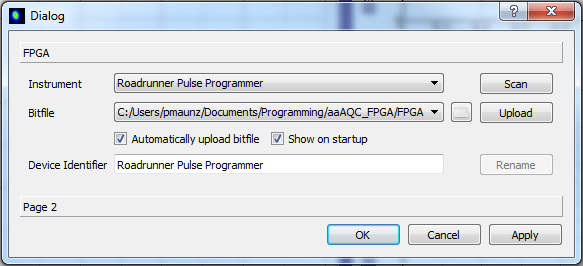
\includegraphics[width=0.7\textwidth]{FPGASettings}
\end{center}
\caption{\label{FPGASettings} FPGA settings window.}
\end{figure}
The FPGA settings window (figure\ref{FPGASettings}) is sown on start-up. If "Automatically upload bitfile" is checked, the bitfile will be uploaded on "OK" otherwise, the bitfile has to be explicitly loaded by pressing {\em upload}. The bitfile can also be uploaded manually. In the case the Instrument selection is empty, please make sure previous processes have been closed (and orphans have been closed). Disconnecting and re-connecting the USB cable should help too. After fixing the problem press "Scan".

\subsection{Plot display}
\begin{figure}[htbp]
\begin{center}
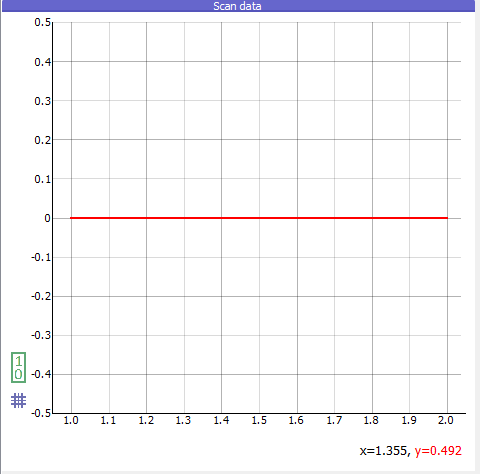
\includegraphics[width=0.8\textwidth]{ScanData}
\end{center}
\caption{\label{ScanData} Plot widget. The A button autoscales the axis, the grid button toggles the grid lines and the "1 0" button scales the vertical axis to a unity range.}
\end{figure}
All plots are displayed using the pyqtgraph library. A typical window is shown in figure~\ref{ScanData}. The scales can be changed dynamically using the mouse. The middle mouse button can be used for panning, the mouse wheel for zooming in and out. If the wheel is used left of the vertical axis (or below the horizontal axis) the vertical axis, (horizontal axis) is zoomed while the other axis remains in autoscale. The "1 0"button on the left sets the vertical axis to a unity scale. The grid symbol toggles the grid display. The current cursor position is shown on the bottom right. The precision of this display can be increased by first zoomin in.


\subsection{Dedicated Counters}
\begin{figure}[htbp]
\begin{center}
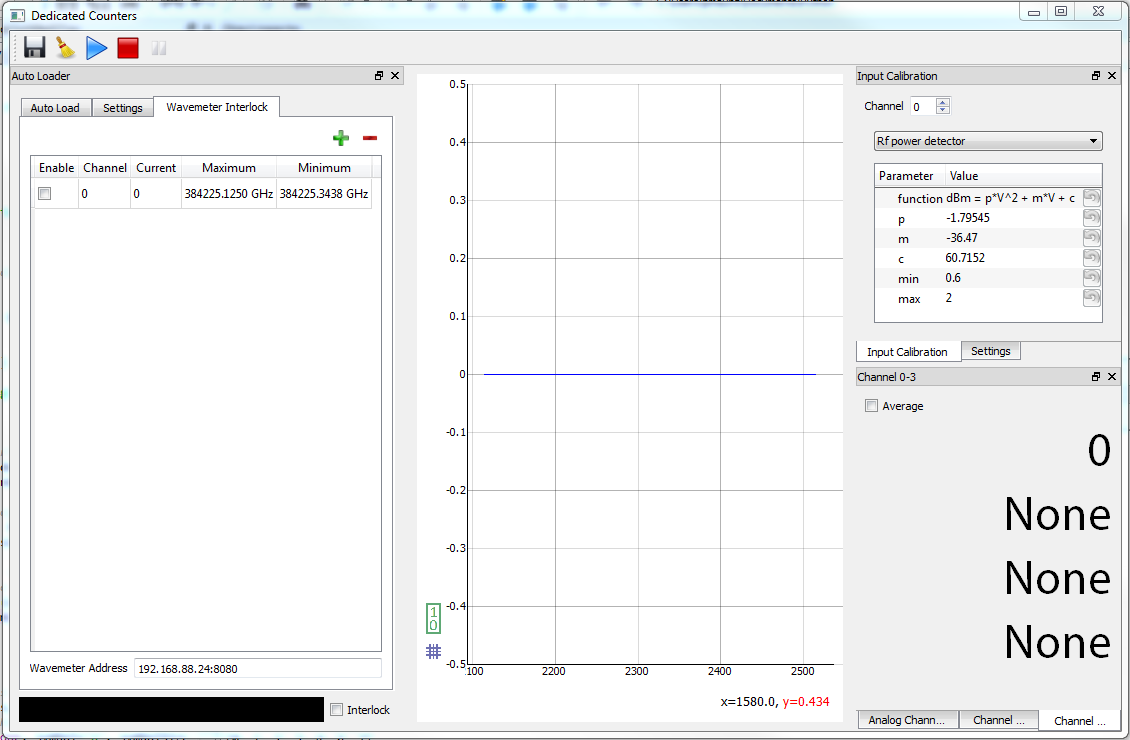
\includegraphics[width=\textwidth]{DedicatedCounters}
\end{center}
\caption{\label{DedicatedCounters} Dedicated counters window. The left dock widget controls the Auto-loading feature. The right dock widgets display the last counter values and analog input values as well as the counter control and input calibration widgets. Dock widgets can be re-arranged, torn out or closed if not needed. }
\end{figure}
In addition to the Pulse Program, the FPGA has dedicated counters for all $8$ digital input lines and $4$ analog inputs. These counters are {\em not} synchronized with the execution of the Pulse Program, nor do they stop during the Pulse Program execution. The analog input channels can be calibrated to display voltage or any function can be used to map the values to different quantities. Currently there is a conversion function for reading the Mini-Circuits rf-power detectors. Others can be added easily.

The dedicated counters and  the Auto-load feature building upon it are controlled from the "dedicated counters" window (figure~\ref{DedicatedCounters}). 

The counter channels can be selected from the controls shown in Figure~\ref{DedicatedCountersSettings}. Points to keep determines how many points are kept, and the integration time can be adjusted. There are glitches in the displayed values when the integration time is changed.

\begin{SCfigure}
\centering
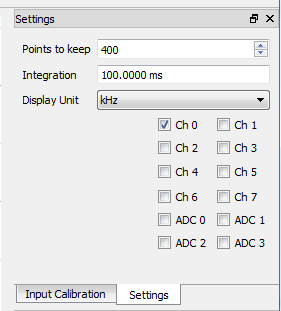
\includegraphics[width=0.5\textwidth]{DedicatedCountersSettings}
\caption{\label{DedicatedCountersSettings} Counter control widget. The $8$ digital and $4$ analog input channels can be selected independently. The integration time (to be entered with unit) determines the integration time per point. The minimal recommended value is $10\unit{ms}$. }
\end{SCfigure}


\subsection{Autoload}
\begin{figure}[htbp]
\centering
\includegraphics[width=0.48\textwidth]{Autoload}\hfill
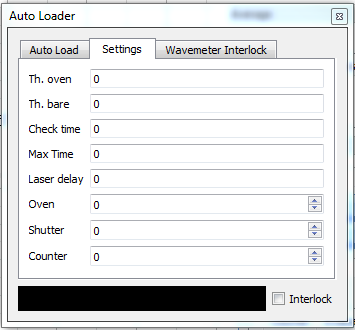
\includegraphics[width=0.48\textwidth]{AutoloadSettings}
\caption{\label{Autoload} Autoload top window (left) and settings window (right). The timer counts the time from beginning of loading during loading. Then it switches to the time since the ion was first detected. A list of historic times is kept. Loading time is the time from switching on the oven to the detection of an ion. Trapping time the time between first detection and the last time the ion was detected.}
\end{figure}
The auto-load feature allows automated loading where the counts on one counter and optionally the wavelength from a Highfinesse wavemeter are checked.

\paragraph{Settings}
The Auto-loading feature takes the input of one counter channel as plotted in the dedicated counters window. The main loading window is shown in figure~\ref{Autoload}. The settings controlling the auto-load feature are entered in the Settings tab. The loading is done with the following steps: 
\begin{description}
\item[\lit{Preheat}] The oven is on, the loading laser blocked. No ion detection is performed. After \lit{Laser delay} time, it will proceed to \lit{Load}.
\item[\lit{Load}] The oven and loading lasers are on. Is the ion detected the state will proceed to \lit{Check}. Is \lit{Max time} reached, auto-loading fails and is stopped.
\item[\lit{Check}] Oven and laser are off, if the ion is not detected, the state is set to \lit{Load}. After the \lit{Check time}, the state proceeds to \lit{Trapped}.
\item[\lit{Trapped}] If the ion is not detected the state is set to \lit{Disappeared}.
\item[\lit{Disappeared}] If the ion is found back during \lit{Check time} the state is set to \lit{Trapped}.
\end{description}
These settings are as follows:
\begin{description}
\item[\lit{Th. oven}] Threshold for detecting an ion while the oven is on (allows to compensate in case oven operation leads to additional scatter). The threshold is given in counts per integration time. To be entered with frequency unit.
\item[\lit{Th. bare}] Threshold bare. This is the threshold used if the oven is off.
\item[\lit{Check time}] After an ion is detected, the ion has to be detected for at least this time. If the ion leaves during this time
\item[\lit{Max Time}] Maximum time the oven is on. Even with multiple cycles between \lit{Check} and \lit{Load} states, this time is not exceeded.
\item[\lit{Laser delay}] Delay time after which the loading laser is switched on (preheat time).
\item[\lit{Oven}] Shutter bit number of the oven enable bit. 
\item[\lit{Shutter}] Shutter enable bit of the loading laser shutter.
\item[\lit{Counter}] Counter channel to be used for ion detection.
\end{description}

The autoload feature is disabled while a pulse program is running. In addition, starting a pulse program will interrupt the loading process. This is necessary because the autoload feature cannot control the shutter output bits while a pulse program is running.

\paragraph{Interlock}
In addition to observing the counts it is possible to monitor relevant laser frequencies and stop the loading process if a laser is out of lock. The interface is shown in figure~\ref{WavemeterInterlock}.
\begin{SCfigure}
\centering
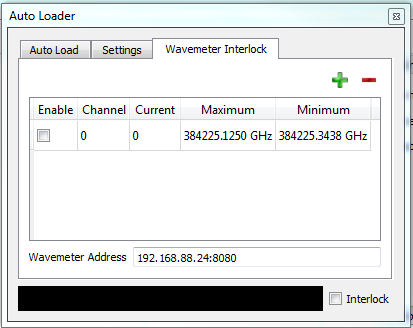
\includegraphics[width=0.6\textwidth]{WavemeterInterlock}
\caption{\label{WavemeterInterlock} Wavemeter interlock. The address of the wavemeter control computer is entered at the bottom, it has to contain only the host name and optionally the port number. Individual channels can be added or removed with the plus or minus button, respectively. Maximum and Minimum are always entered in GHz.}
\end{SCfigure}

The inerlock queres the wavemeter periodically. Is the wavelength out of the given range for $10$ consecutively queries, the loading process is stopped if the Interlock is enabled (checkbox on lower right). The bar at the bottom of the window is black for disable interlock, red if at least one laser is out of range and green if all lasers are in range.

\subsubsection{Analog Inputs}
The voltages at the analog inputs can be either displayed in Volt or converted. This is used for example to convert the reading from a Mini-Circuits power detector from voltage into rf power. The configuration of these input calibrations is controlled by the window shown in figure~\ref{AnalogInputCalibration}. The fit parameters for the Mini-Circuits power detector can be entered here. Additional input calibrations can be easily defined by deriving a class from the class \lit{AnalogInputCalibration} in the file \lit{AnalogInputCalibration.py} and adding the new class to the dictionary \lit{AnalogInputCalibrationMap} also defined in the same file. There is no additional gui programming necessary to add additional calibrations.

\begin{SCfigure}
\centering
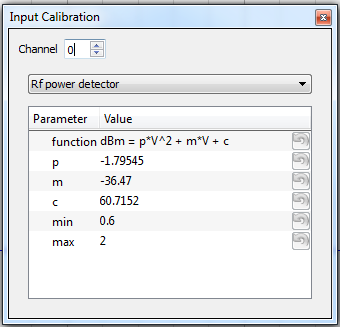
\includegraphics[width=0.5\textwidth]{AnalogInputCalibration}
\caption{\label{AnalogInputCalibration} Analog input calibration. The calibration can be selected for each channel. Additionally, the calibration can define parameters which are entered here.}
\end{SCfigure}

\subsection{Global Variables}
\begin{SCfigure}
\centering
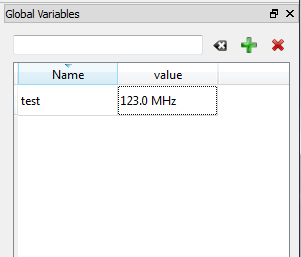
\includegraphics[width=0.5\textwidth]{GlobalVariables}
\caption{\label{GlobalVariables} Global variables window. Global variables can be defined here. The value should be entered with dimensions. Entering of mathematical expressions is possible, however the expression will only be evaluated once and replaced with the result. The variables can be sorted by name, or re-ordered be hand: selected rows can be moved up or down by pressing the Page-Up and Page-Down keys, respectively. New variables are added by entering the name and clicking the plus icon.}
\end{SCfigure}

Global variables can be defined as shown in figure~\ref{GlobalVariables}. These variables can then be used in all Pulse Program controls.

\subsection{Static settings}
Static settings are the settings that are applied while no Pulse Program is running. In this case the shutter values, trigger values and DDS settings can be controlled by the respective control dock windows.

\subsubsection{DDS}
\begin{SCfigure}
\centering
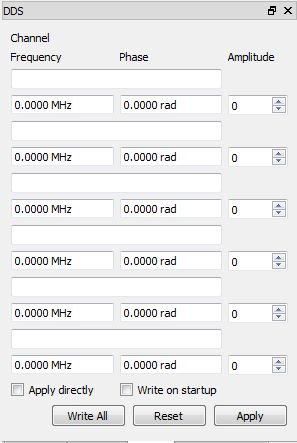
\includegraphics[width=0.5\textwidth]{DDS}
\caption{\label{DDS} DDS control window for 6 DDS channels. The channel names are for the memory of the user. The frequency has to be entered with a frequency unit. The Phase has to be entered with the unit rad. (Please excuse that in most other parts the phase is entered in degree and without unit). The amplitude is entered as an integer between 0 and 1023. If apply directly is checked, the io-update signals are generated after each change. If it is not checked, the apply button has to be clicked. Reset triggers a channel reset, values have to be written explicitly thereafter. }
\end{SCfigure}
The DDS settings are entered in the window show in figure~\ref{DDS}.  The channel names are only for the memory of the user. These values are {\em not} used anywhere else. The frequency has to be entered with a frequency unit. The Phase has to be entered with the unit rad. (Please excuse that in most other parts the phase is entered in degree and without unit). The amplitude is entered as an integer between 0 and 1023. If apply directly is checked, the io-update signals are generated after each change. If it is not checked, the apply button has to be clicked. Reset triggers a channel reset, values have to be written explicitly thereafter. The controls are disabled while a Pulse Program is running. After the execution of a Pulse Program, the DDS chips might be left at different settings. In the configuration of Pulse Program scans an option to automatically write the static settings can be selected.

The fields for frequency and phase can be changed by pressing the up and down keys. The value is then increased or reduced by the value of the digit left of the cursor.

\subsubsection{Shutters}
Shutters are the digital outputs of the system. These can be toggled by clicking the red (off, low) or green (on, high) field. The channel name that can be entered in the left column is only for the reference of the user and defines the shutter names shown in the Pulse Program and Logic Analyzer windows.

\begin{SCfigure}
\centering
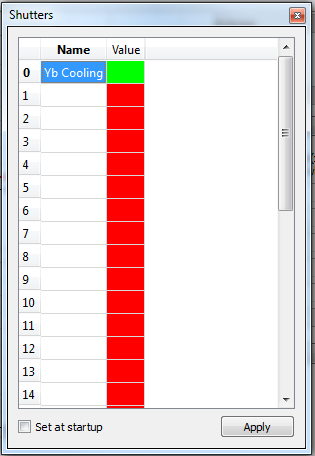
\includegraphics[width=0.4\textwidth]{Shutters}
\caption{\label{Shutters} Shutter control. Channel names can be entered on the left, the output toggled on the right. The control is disabled while a Pulse Program is running.}
\end{SCfigure}

\subsubsection{Triggers}
The triggers are digital outputs that are low by default and only switched to high for one clock cycle. The control window is similar to the Shutter window. Only here "not triggered" is represented by a white field. Triggers are applied by clicking Apply.

\subsection{External Instruments}
External instruments include all external instruments connected via GPIB, USB, Serial, IP-network to the host computer. The external instruments have one value that can be controlled and used for scans. In addition each instrument can define a number of Parameters which can be controlled from the gui. The External parameter interface consists of two windows: "Params selection" and "Params control". Params selection serves to establish a connection to the device and control the Parameters. The Paras control window combines the main channels of all enabled External Instruments.

\subsubsection{External Instrument Selection}

\begin{SCfigure}
\centering
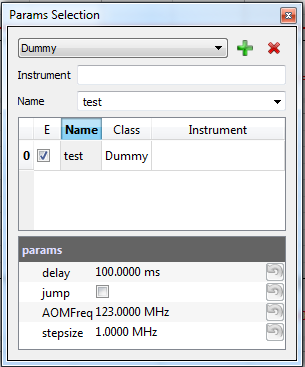
\includegraphics[width=0.5\textwidth]{ParamsSelection}
\caption{\label{ParamsSelection} Parameter selection window. The top selection box lists the available instrument classes. The connection information has to be entered in the \protect\lit{Instrument} field. The \protect\lit{name} serves to identify the devices and has to be unique. Clicking the plus icon will add a new instrument with these settings to the list. When the checkbox in the first column is checked a connection is established.}
\end{SCfigure}

The available instruments are configured in "Params Selection" (figure~\ref{ParamsSelection}). A connection to the device is only established once the check box in the first column is checked. When clicking on an active row, the parameters of the device can be changed in the lower list. All instruments inherit the \lit{stepsize}, \lit{delay}, and \lit{jump} settings. These are meant for values (as for example lasers locked to sideband generated by a synthesizer) that may only be changed in steps. The generated steps are of size \lit{stepsize} and are executed with a delay of \lit{delay} between consecutive steps. Checking \lit{jump} will deactivate this feature and apply values directly.

The \lit{dummy} instrument is used for debugging.

The order of the instruments can be changed by selecting rows and pressing the \lit{Page-Up} or \lit{Page-Down} keys to move the selected row up or down, respectively.

Additional instruments can be added without gui programming by deriving a class from the class \lit{ExternalParameterBase} in file \lit{ExternalParameter.py}. The newly generated class has to be added to the \lit{ExternalParameter} dictionary which is defined at the bottom of the the same file.

\subsubsection{External Instrument Control}

\begin{SCfigure}
\centering
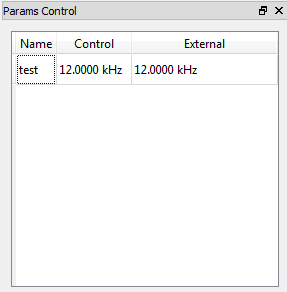
\includegraphics[width=0.5\textwidth]{ParamsControl}
\caption{\label{GlobalVariables} Parameter control window. The main value of all active instruments is controlled from here. The order follows the order of the instruments in the "Params selection" window. The control column is editable and used to change the current value. The External column reports the value as last written or reported by the device (if possible).}
\end{SCfigure}
This window combines the main values of all external instruments. The order follows the order of the instruments in the "Params selection" window. The control column is editable and used to change the current value. The External column reports the value as last written or reported by the device (if possible). Should a connection be lost, try disabling and enabling the instrument in the "Params selection" window.


\section{Pulse Program}
The Pulse Program window serves as graphics interface to the pulse program. A pulse program is loaded with the "File open" button. The selection box gives easy access to recently used pulse programs. The system remembers the path of the file internally. Thus using files of the same filename at different locations will be confusing and is discouraged. The values of variables defined in the pulse program are shown in the interface. The variables in the gui {\em overwrite} the values defined in the pulse program (Figure~\ref{PulseProgram}). 
\begin{figure}[htbp]
\begin{center}
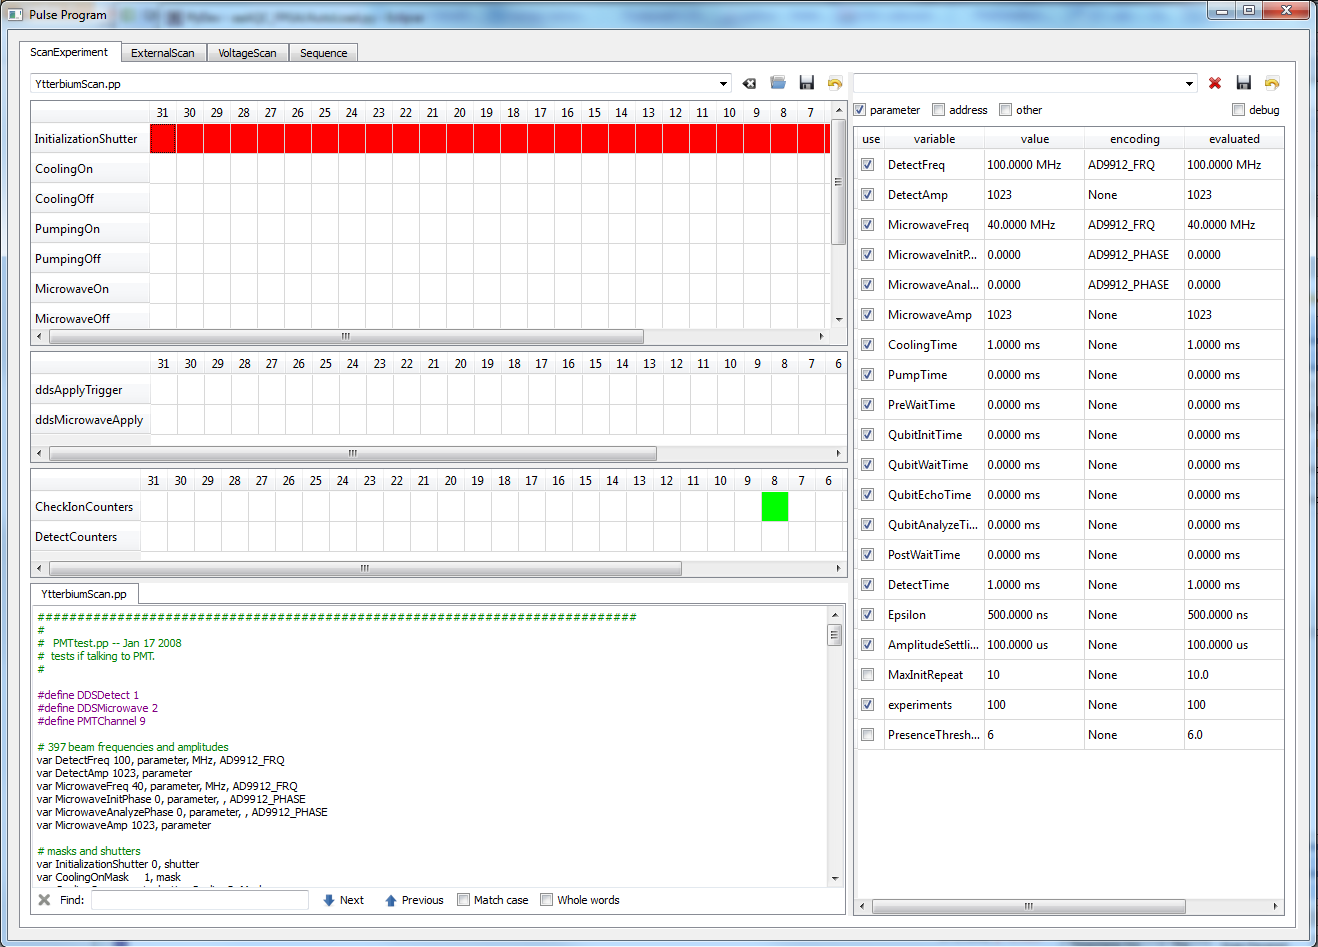
\includegraphics[width=\textwidth]{PulseProgram}
\end{center}
\caption{\label{PulseProgram} Pulse Program window. There is a tab for every pulse program used by the different measurement tabs of the Main Window.}
\end{figure}

The interface to the shutter values (top left) combines shutter_mask and shutter variables. The table on the left allows to change the trigger values, the third window allows to control the counter gates.
Currently, the $8$ input channels are routed to counters $0-7$, $8-15$, $16-23$, and to the time-stamping circuits $24-31$.
The accumulated counts from channels $0-15$ are transmitted back to the computer when the gate is closed. Channels $16-23$ are only accessible from the pulse program. Channels $24-31$ lead to the transmission of a time-stamp for every detected pulse. The time resolution of $20\unit{ns}$ is given by the FPGA clock frequency $50\unit{MHz}$.

The control for the variables can be found on the right. The "use" column allows one to set the variable to $0$ while keeping the previous value in the value field. The value field accepts mathematical expressions including dimensions and can reference local and global variables. The program will prevent the definition of cyclic dependencies.

The values in the gui are saved in the gui configuration file. The pulse program file is saved exactly as shown in the bottom left. An external editor can be used.

\section{Scan configuration}
The Scan configuration allows the user to control how the scan is executed and evaluated. All values are copied when the scan starts. Changes to any of these controls will only go into effect for newly started scans. The window is how in Figure~\ref{ScanParametersScan}. All scan settings can be saved under a name that is entered in the selection box at the top. The current values are saved under this name when the "save" button is pressed. The "reload" button allows to re-load the values that were saved before under the name currently showing in the selection box. Selecting a different saved set from the selection box will load those values.
The undo and redo button go back to the last set of values used for the last executed scan.

\begin{SCfigure}
\centering
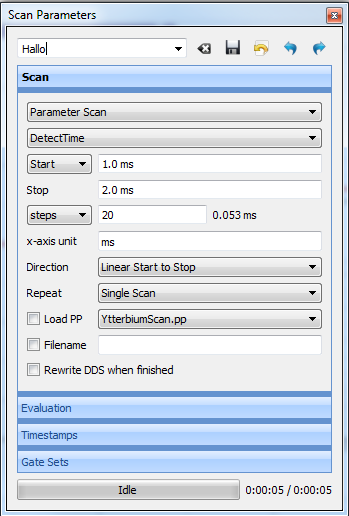
\includegraphics[width=0.5\textwidth]{ScanParametersScan}
\caption{\label{PulseProgram} Scan Control --- Scan. A scan is defined here. \protect\lit*{Parameter Scan} will overwrite one of the variables in the pulse program, \protect\lit*{Step in Place} will repeat the experiment as defined in the pulse program. In this case, he number of steps defines how many points are kept.  \protect\lit*{Gate Sequence Scan} will scan through the values defined in the Gate Sequence configuration files.}
\end{SCfigure}
\subsection{Scan settings}
The  way he scan is executed is defined in the \lit*{Scan} tab. The possible scans are:
\begin{description}
\item \lit*{Step in place} which will execute the current pulse program repeatedly with the same settings.
\item \lit*{Parameter Scan} will overwrite the variable from the current pulse program selected in the next selection box. If the value that was last selected is not available in the current pulse program, it will be displayed in red. 
\item \lit*{Gate Sequence} Allows to scan over different gate sequences as defined in the gate sequence configuration files.
\end{description}
The scan can be defined with start and stop values or center and span values. In addition either the number of steps or the stepsize can be defined. The x-axis unit defines the unit to which values are converted before they are plotted. The scan direction can be either \lit*{Linear Start to Stop}, \lit*{Linear Stop to Start} and \lit*{Randomized}. Randomized will execute the different points in a random permutation defined at the beginning of the scan. Results are saved in the order the points were taken. If \lit*{Load PP} is checked, the pulse program file selected on the right is loaded when the scan control settings are loaded. If \lit*{Filename} is checked, results will automatically saved to the filename given on the right. If only a filename is given, the data will be saved under this filename once the user presses the save button in the Trace user interface. When saving, a three digit serial number is inserted before the last period of the string given in \lit*{Filename}.

\subsection{Evaluation settings}
\begin{SCfigure}
\centering
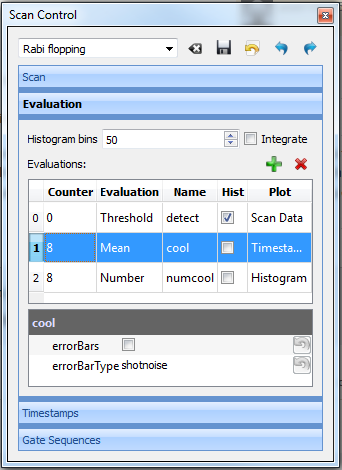
\includegraphics[width=0.5\textwidth]{ScanParametersEvaluation}
\caption{\label{PulseProgram} Evaluation definition.}
\end{SCfigure}
The way the count values from the different channels are evaluated is defined in the \lit*{Evaluation} tab. Pressing the plus icon will add a new evaluation, pressing the minus icon will delete currently selected evaluations. After adding, the different fields can be changed. The Counter channel which counter channels is evaluated. The Evaluation defines the kind of evaluations. It is easy to add newly defines evaluations. A unique Name is necessary for identification. If Hist is checked a histogram will be displayed in the Histogram graph. Plot defines in which plot window the results are displayed. Available evaluations are:
\begin{description}
\item \lit*{Threshold} Does a simple thresholding, where the threshold value is entered in the parameter window (after selection the evaluation). A value of $n$ means count values $0-n$ are considered dark, count values $>n$ are considered bright. Error-bars are  represent the Wilson score interval with continuity correction\footnote{see http://en.wikipedia.org/wiki/Binomial_proportion_confidence_interval}. These are always limited by 0 and 1.
\item \lit*{Mean} Evaluated to the mean count number. Error-bars can either be shot-noise $\sqrt{\sum_{i=1}^N{x_i}}/N$ or statistical standard error $$\frac{1}{\sqrt{N-1}}\sqrt{\langle x^2 \rangle - \langle x \rangle^2},$$ where $N$ is the number of values averaged.
\item \lit*{Number} Evaluated to the number of count values received. This is useful if a loop in the pulse program leads to a variable number of results in a channel.
\end{description}

\subsection{Time-stamp settings}
The time-stamp settings define how time-stamps are displayed. If enabled, the binwidth defines the time-interval combined into one value. This values should be chosen in multiples of the clock duration ($20\unit{ns}$). ROI start defines the start of the plot with respect to the gate. ROI width the width of the curve shown. Counter defines which counter values are displayed. Here $0-7$ corresponds to the pulse program countermask in bits $24-31$. 
\begin{figure}[htbp]
\begin{center}
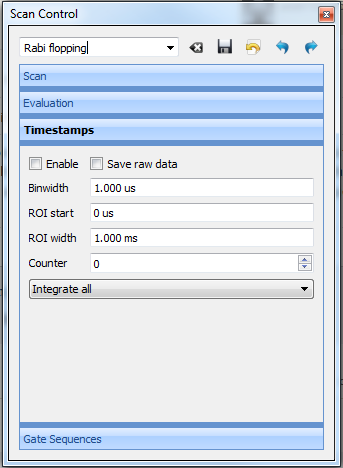
\includegraphics[width=0.5\textwidth]{ScanParametersTimestamps}
\end{center}
\caption{\label{PulseProgram} Main window.}
\end{figure}


\subsection{Gate Sets settings}
\begin{figure}[htbp]
\begin{center}
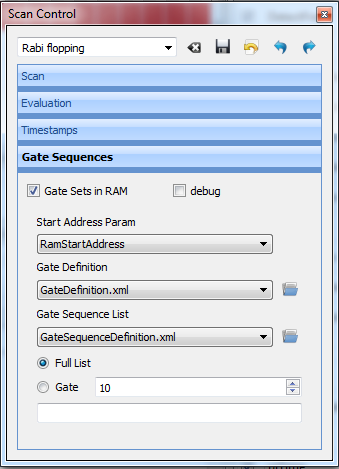
\includegraphics[width=0.5\textwidth]{ScanParametersGateSequences}
\end{center}
\caption{\label{PulseProgram} Main window.}
\end{figure}

\section{Logic Analyzer}

\section{Curve fitting}
\begin{figure}[htbp]
\begin{center}
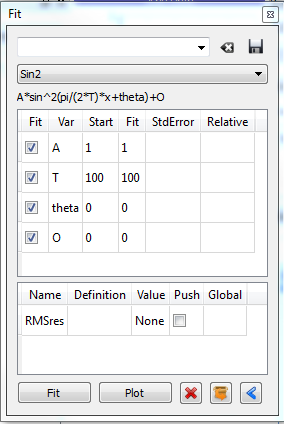
\includegraphics[width=0.5\textwidth]{CurveFitting}
\end{center}
\caption{\label{AutoloadSettings} Main window.}
\end{figure}

\section{Traces}
\begin{figure}[htbp]
\begin{center}
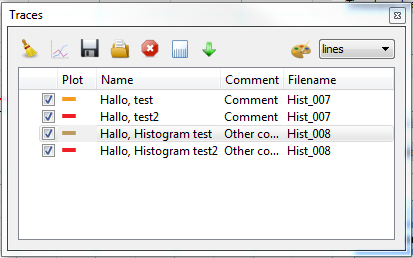
\includegraphics[width=0.5\textwidth]{Traces}
\end{center}
\caption{\label{AutoloadSettings} Main window.}
\end{figure}

\section{Extending the program}

\subsection{Analog Inputs}

\subsection{External Parameters}

\subsection{Count evaluation}

\subsection{Fit functions}

\end{document}